\section{Desarollo packet pincer}

En esta sección veremos el funcionamiento de cada parte de la herramienta, la cual se ha llamado 'packet pincer' por el momento. Veremos qué y cuáles argumentos de consola acepta, como realiza la lectura de paquetes tanto en tiempo real como por trazas. A continuación se explicarán los diferentes pasos que llevan a cabo en el momento al analizar un paquete y como se realiza la generación de estadísticas. Finalmente, veremos como se realiza el etiquetado automático de los flujos y se escriben emiten los resultados.

Un esquema del flujo principal de la aplicación se puede observar en la Figura \ref{fig:packetpincerexecution}. Como podemos ver, se van extrayendo paquetes mientras se encuentren disponibles. Cuando se obtiene uno, en caso de ser un paquete IPv4 fragmentado, se intenta reconstruir o se guarda en caso de no poder. A continuación, se comprueba si la herramienta soporta analizar el paquete indicado y, en caso afirmativo, acumula la información en el flujo de transporte respectivo. Finalmente, se 'cierran' los flujos antiguos, es decir, se emite la información relevante y a continuación se descarta el resto de información acumulada.

\begin{figure}[H]
  \begin{center}
    \centering
    \resizebox{!}{\dimexpr\textheight-2\baselineskip\relax}{%
      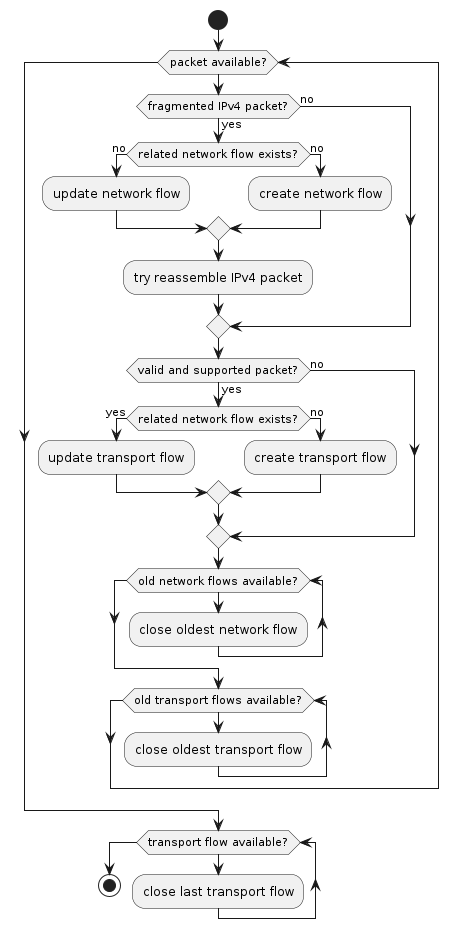
\includegraphics{plant_uml_diagrams/general_tool_loop.png}
    }
  \end{center}
  \caption{Flujo de la aplicación durante su ejecución}\label{fig:packetpincerexecution}
\end{figure}

\subsection{Argumentos y señales}

El programa está pensado para ser ejecutado desde el terminal. Debido a esto, hemos de definir que argumentos se pueden pasar al programa y hacer que este reaccione a señales del sistema operativo. Los argumentos suelen ser pasados desde el mismo comando utilizado para ejecutar el programa, siendo un ejemplo '\texttt{packet\_pincer \underline{help}}'. Las señales a su vez se pueden enviar utilizando una combinación de teclado como \texttt{CTRL+C} o utilizando otro programa.

Para hacer la gestión de los argumentos enviados por el terminal, se ha hecho uso de la librería (o 'crate', en la nomenclatura utilizada en Rust) clap \cite{Knapp_clap_2024}. Concretamente, se ha hecho uso de la funcionalidad 'derive', la cual permite expresar los argumentos a pasar como un tipo del lenguaje de forma declarativa. Adicionalmente, la librería añade diversas funcionalidades que mejoran la experiencia de usuario. A partir de nuestras definiciones, se muestran unas indicaciones de uso si se ejecuta \texttt{packet\_pincer --help} o si se pasan argumentos inválidos. Los argumentos definidos para el programa consisten en:

\begin{enumerate}
  \item Opcionalmente indicar si escribir los resultados generados en archivos (indicando su prefijo), en la salida estándar o no emitir nada.
  \item Opcionalmente indicar si un archivo en formato csv de las etiquetas que han de ponerse en los flujos. En caso de que se especifique este archivo y no haya etiqueta correspondiente, se generará una llamada 'benign'.
  \item Indicación del origen de los paquetes a analizar. Este puede ser 'offline' (a partir de una traza de red o un directorio de estas) u 'online' (a partir de una interficie de red).
\end{enumerate}

Respecto a las señales, se hace uso de la librería ctrlc \cite{controlc}. Esta permite detectar señales de interrupción enviadas por el usuario para interrumpir la ejecución de la aplicación. Si el programa no respondiese a estas señales, el sistema operativo terminaría el proceso directamente. Esto podría provocar la escritura parcial de los archivos, potencialmente corrompiéndolos. En caso de que se genere una señal de interrupción del programa, lo tratamos como que no hay más paquetes disponibles.

El código que se encarga de tratar estos puntos, se puede encontrar en \texttt{main.rs} en el anexo 2 o en el repositorio de GitHub.

\subsection{Lectura de paquetes}

\subsubsection{Librerias}

Para realizar la lectura de paquetes, tanto en tiempo real como a partir de archivos, se ha escogido hacer uso de la librería de rust 'pcap' \cite{rustpcap}, la cual a su vez hace uso internamente de otra llamada 'libpcap' la cual es desarrollada por el grupo tcpdump \cite{libpcap}. Dependiendo de si queremos leer paquetes desde un archivo o desde una interfaz de red, tendremos que utilizar una función de la API pública u otra para generar una instancia 'Capture'. 

\subsubsection{Detalles de implementación comunes}

A pesar de que la librería ofrece casi todas las funcionalidades que se requieren, no ofrece soporte para leer desde una lista de archivos, sino que hemos de leer de cada uno individualmente. Debido a esto, se ha creado la envoltura 'PacketCapture' disponible en \texttt{packet\_capture.rs} en el anexo 2 o en el repositorio de GitHub. En esta, se permite crear una instancia a partir de una ruta, que puede ser un archivo, un directorio o una interfaz de red. Adicionalmente, permite al usuario del módulo hacer una petición para procesar el siguiente paquete. Esto se hace a través de pasar una clausura que acepta un 'PacketOrigin' (ruta del archivo o nombre, interfaz), un 'LinkType' (el tipo de la capa de enlace \cite{linktypetcpdump}) y una referencia al paquete a tratar. La función de procesamiento extrae el siguiente paquete y llama a la clausura, devolviendo un valor afirmativo si se ha podido extraer un paquete o un valor negativo en caso de contrario.

Se hace uso de una clausura en vez de devolver una referencia al paquete debido a que el compilador no lo permitía. Después de investigar, esto era causado por el hecho que la librería pcap, dentro de la instancia 'Capture', tenía una referencia a un trozo de memoria. Al seguir manteniendo una referencia a la captura después de ejecutar la función, esto causaba que el compilador no pudiese garantizar que esta referencia fuese válida. En cambio, al pasar una clausura se puede asegurar a que se haga un uso correcto de la memoria al poder indicarlo en el prototipo de la función proporcionada por el usuario del módulo.

\subsubsection{Lectura de paquetes en tiempo real}

Para el caso de la lectura de paquetes en tiempo real, podemos hacer uso relativamente directo de la librería. En el momento de crear 'PacketCapture' creamos la instancia 'Capture' basada en una interficie de red. Cuando queremos procesar el siguiente paquete, pasamos la petición directamente a 'Capture' y a continuación ejecutamos la clausura. Si no hay errores, devolvemos un valor verdadero, indicando que hay potencialmente más paquetes válidos. En caso contrario, indicamos un valor negativo, indicando que probablemente no se puedan capturar más paquetes.

\subsubsection{Lectura de trazas de paquetes}

El caso de la lectura de trazas es más complicado. Debido a que se quiere admitir el poder leer de uno o varios archivos, es necesario hacer una mayor gestión adicional a la que nos proporciona la librería. Para esto, se han definido tres estructuras internas:
\begin{enumerate}
  \item \textbf{OwnedPacket}: Un paquete el cual 'posee' la memoria a la que hace referencia. A diferencia del que nos proporciona la librería pcap, no hace referencia a una sección de memoria que puede formar o no parte de otra mayor, permitiéndonos garantizar que las referencias a memoria son válidas.
  \item \textbf{FileCapture}: Una envoltura de una 'Capture' de la librería pcap con su ruta de origen y el siguiente paquete que se debe tratar extraído. Esto se hace para poder ordenar las diferentes 'FileCapture' según el tiempo de captura del paquete.
  \item \textbf{FileCaptureCollection}: Un conjunto de 'FileCapture'. Está estructurado en dos campos: un 'HashMap' de la librería estándar y en una cola de prioridad \cite{priority-queue}. El primero es utilizado para poder acceder en tiempo constante a cualquier 'FileCapture' a partir de su ruta y el segundo para tener una lista ordenada de más a menos antiguo del siguiente paquete a analizar. Esto es necesario debido a que hay algunos conjuntos de datos contienen archivos que se solapan en el tiempo.
\end{enumerate}

Para generar la instancia a partir de la ruta, navegamos por todos los archivos y directorios de esta haciendo uso de walkdir \cite{walkdir}. Por cada archivo, intentamos abrirlo como captura pcap y, en caso de no ser posible, lo saltamos. Una vez abierto, extraemos el primer paquete de la captura y creamos un 'FileCapture' con las tres partes necesarias. Finalmente, creamos el 'HashMap' con todas las capturas abiertas y la cola de prioridad para poder acceder a las capturas de forma ordenada.

Para procesar el siguiente paquete, primero se obtiene la ruta de la captura con el siguiente paquete más antiguo. A continuación, se encuentra la instancia 'FileCapture' y llamamos a la clausura con esta. Una vez hecho esto, se trata de extraer el siguiente paquete de la traza de red. En caso de error, eliminamos la captura tanto de la cola como del 'HashMap'. En caso contrario, actualizamos el valor del siguiente paquete en 'FileCapture' y su posición en la cola.

\subsubsection{Obtención de paquetes} \label{obtencionpaquetes}

El uso de la envoltura \texttt{PacketCapture} se realiza desde \texttt{main.rs} disponible en el anexo 2 y en el repositorio. Una vez creada a partir de los argumentos proporcionados, se define una clausura para proporcionarlas a la función de procesamiento. A continuación se hace uso de un bucle infinito que llama a la función \texttt{try\_process\_next} en \texttt{PacketCapture}, pasando la clausura como argumento. Esto se realiza hasta que la función devuelve un valor falso o se reciba una señal de terminación. Dentro de la clausura, se acumula información en una instancia de \texttt{FlowGroup} (donde se decodifica el paquete y se acumula la información relevante del paquete), se actualizan las estadísticas de ejecución y se emiten estadísticas de flujos finalizados.

\subsection{Decodificación de paquetes y extensión de librería de código abierto} \label{packetdecode}

\subsubsection{Análisis librería}

Los datos ofrecidos por la librería \texttt{pcap} consisten en información de cuándo se capturó el paquete, cuál era la capa de enlace y los datos en crudo capturados. Es decir, nos interpreta exclusivamente la parte del formato 'libpcap' vista en \ref{libpcapformat}. Para interpretar el resto de capas indicadas en \ref{netformats}, haremos uso de la librería \texttt{etherparse} \cite{etherparse}.

Después de un primer análisis, se observó que la librería soportaba interpretar tramas de Ethernet \ref{etherformat}, paquetes IP \ref{ipformat}, datagramas UDP \ref{udpformat} y segmentos TCP \ref{tcpformat}. Sin embargo, no ofrecía soporte para SLL \ref{sllformat}, el cual necesitábamos para el dataset TON-IoT. Debido a que la librería tenía soporte para la mayoría de puntos necesarios, además de ofrecer una interfaz sencilla, se decidió hacer una extensión de esta para añadirle soporte de SLL. 

\subsubsection{Extensión librería}

Para realizar esto, primero se creó un 'issue' en el repositorio original el 24 de abril de 2024 para indicar al desarrollador de la librería sobre la intención de hacer esta adición \cite{slladdsllissue}. No se recibió respuesta, pero se inició el trabajo para añadir el soporte. Durante los siguientes 5 días, se añadieron 4,145 líneas de código y se eliminaron 141. En estas, se incluye el formato SLL, el proceso para extraer los valores relevantes desde datos en crudo desde el formato SLL, tests y toda la documentación asociada. Se trató de mantener el estilo de la librería para asegurar que el desarrollador original aceptaría los cambios. Una vez finalizado, el 29 de abril se creó un 'pull request' para juntar los cambios \cite{slladdsllpr}. En esta instancia, el desarrollador contestó agradeciendo el trabajo realizado. Después de que lo revisara y arreglase algunos detalles de integración, el 2 de mayo juntó los cambios a la rama principal.

\subsubsection{Uso de la libreria}

El primer uso durante el flujo del programa es en la función \texttt{try\_parse\_packet} disponible en \texttt{packet\_parse.rs} en el anexo 2 o en el repositorio. La función se llama después de realizar la extracción de un paquete desde \texttt{PacketCapture} o después de hacer una reconstrucción como veremos en \ref{ipv4defrag}. Dentro de la función, a partir del tipo de capa de enlace indicado por \texttt{pcap} y la librería etherparse, obtenemos una instancia de \texttt{SlicedPacket} de la cual podemos obtener los campos de diferentes capas del paquete original. En caso de datos Ethernet, utilizamos la función \texttt{etherparse::SlicedPacket::from\_ethernet} y en caso de tener datos en SLL, hacemos uso de {etherparse::SlicedPacket::from\_linux\_sll} añadida durante el desarrollo del proyecto.

\subsection{Obtención de identificadores} \label{idextraction}

Como se indicó en los puntos anteriores, después de obtener un paquete tratamos de primero decodificarlo y acumular la información relevante. Para poder hacer una diferenciación de las diferentes comunicaciones, extraemos un 'identificador del flujo' para poder clasificarla.

En la herramienta, consideramos dos casos de identificadores. Primero, un 'identificador de red', el cual usamos en los paquetes que portan un paquete IPv4 fragmentado. Para la identificación, hacemos uso de las direcciones de origen y destino, además del campo 'identifier' disponible en la cabecera IPv4. A continuación, un 'identificador de transporte', el cual es utilizado cuando tratamos con un paquete IP versión 4 o 6 y porta un datagrama UDP o un segmento TCP. En este caso, utilizamos cinco valores para la identificación. Estos consisten en las direcciones de origen y destino, los puertos de origen y destino y finalmente el identificador del protocolo de la capa de transporte. En caso de no darse uno de los casos considerados, se emite un error indicando la razón (sin capa de red, de transporte o protocolo no soportado).

Una vez obtenido el identificador del paquete, si tenemos un identificador de red, se realiza paso de desfragmentación (\ref{ipv4defrag}). En caso de que tengamos un identificador de transporte o hayamos podido reconstruir el paquete, procederemos a acumular la información en el flujo de transporte respectivo (\ref{flowseparation}).

\subsection{Desfragmentación IPv4} \label{ipv4defrag}

Los datasets utilizados contienen tramos donde hay una gran cantidad de paquetes IPv4 fragmentados. Es posible que estén relacionados con ataques y que, si ofrecemos soporte para la desfragmentación en la herramienta, las estadísticas generadas puedan ser más útiles para la detección de ataques. Para realizar esto, se ha definido una estructura llamada \texttt{NetworkFragmentFlow}, la cual acumula fragmentos IPv4 con información adicional para su posterior reensamblado. Adicionalmente, en el momento de hacer un reensamblado, aparte del paquete reconstruido, se emitirá una estructura \texttt{FragmentReasemblyInformation} con la información adicional acumulada. Los diferentes flujos activos serán agrupados en la instancia \texttt{FlowGrup}, donde adicionalmente tendremos flujos de transporte como veremos en \ref{flowseparation}.

Para hacer la gestión de la desfragmentación de paquetes IPv4, contamos con dos atributos en \texttt{FlowGroup}. Primero tenemos un \texttt{HashMap} para poder acceder en tiempo constante a cualquier flujo de red activo a partir de su identificador. A continuación, contamos con una cola para tener la lista de identificadores ordenada por el primer paquete encontrado para poder ser capaces de descartar flujos con este criterio. Con esto, por cada paquete que obtengamos, encontramos el flujo de red activo con el mismo identificador y lo actualizamos con el paquete obtenido. En caso de no encontrarlo, lo creamos. Adicionalmente, después de realizar la inclusión, comprobamos si podemos reconstruir el paquete. En caso positivo, lo hacemos y eliminamos el flujo tanto de la lista de flujos activos como de la cola.

Para evitar que la memoria crezca sin límites en caso de que no se puedan reconstruir los paquetes, \texttt{FlowGroup} contiene dos funciones para extraer el flujo 'más antiguo', siendo este el flujo el cual su primer paquete es el que tiene la marca de tiempo menor. La primera es incondicional, mientras que la segunda permite indicar una antigüedad mínima respecto del último paquete procesado. Mientras que procesa paquete a paquete, se ha impuesto un límite de un minuto de antigüedad máxima. En el momento de finalización del análisis, los paquetes restantes son descartados. 

Respecto \texttt{NetworkFragmentFlow}, internamente contiene diversos valores. Entre estos, se encuentran el tiempo del primer paquete procesado, el tiempo del último procesado, el tamaño esperado del paquete completo, los bytes del campo de datos de los fragmentos y el recuento total de los fragmentos con sus bytes recibidos. Con esta información, en el momento de hacer la reconstrucción, podemos comprobar si no nos quedan huecos entre los bytes. En caso negativo, utilizamos la última cabecera del paquete recibido y le substituimos el campo de datos por los datos reconstruidos. Adicionalmente, generamos una instancia de \texttt{FragmentReasemblyInformation} con la información adicional acumulada (tiempos, cantidades de paquetes y bytes recibidos en total) para poder tener estadísticas con mayor consistencia.

\subsection{Separación de flujos de transporte} \label{flowseparation}

Para la gestión de los flujos de transporte hacemos algo similar que con los flujos de red de paquetes fragmentados. Para correlacionar paquetes con flujos de comunicación, aparte de extraer los identificados en \ref{idextraction}, se ha de tener en cuenta que las direcciones y puertos origen/destino están invertidos en los mensajes de respuesta.

En el transcurso normal del protocolo TCP existe una finalización de la transmisión explícita. Sin embargo, se ha de tener en cuenta la posibilidad de que la conexión se interrumpa sin esta. Adicionalmente, UDP no tiene ningún tipo de forma de indicar que una comunicación ha terminado. Por tanto, la gestión de considerar que un flujo ha terminado se ha basado en todos los casos en 'timeouts', es decir, se hace de una manera similar al 'descarte' que se realiza para los paquetes fragmentados. A pesar de hacerlo de forma similar, utilizaremos funciones separadas para poder tratar los dos niveles de forma distinta.

Para almacenar la información, también se hace uso de \texttt{FlowGroup}. En este, tenemos un \texttt{HashMap} para tener acceso en tiempo constante a los flujos y una cola de prioridad para mantener un orden temporal. En este caso, el criterio que se sigue consiste en tener los flujos que han tenido una recepción de un paquete más nuevo más atrás de la cola. Es decir, si en el flujo $A$ el último paquete ha sido en $t=10$ y en el flujo $B$ ha sido en $t=5$, el flujo $B$ se encontraría antes del flujo $A$. Cada vez que actualizamos la información de un flujo a partir de un paquete, actualizamos la posición de este para que esté al final de la cola.

\subsection{Generación de estadísticas}

(estadisticas ejecucion)

(estadisticas paquetes)

\subsection{Escritura y etiquetado de flujos} \label{flowwrite}

Por hacer

